\scanpage{56}
\mspage{3}

où maintenant ``spéciaux'' signifie que $\rho_1=\tau_0\tau_\infty$ opère sans points fixes.

Si on a une carte orientée, sa \deleted{\unsure{considérer}} carte duale munie de la \uline{même orientation de la surface sous-jacente commune}, est appelée la \uline{carte orientée duale}. On aura alors
\[
(9)\qquad R^+(\check C)=R^-(C),\quad R^-(\check C)=R^+(C)
\]
i.e. les repères directs pour l'une des deux cartes en dualité sont ceux qui sont inverses pour l'autre.

On se libère de la condition de restriction aux $G_2^\circ$-ensembles finis \uline{spéciaux}, en introduisant une notion un peu plus générale de carte cellulaire, en \deleted{\unsure{admettant des}} \inserted{introduisant la notion} d'\uline{arête pliée} -- Techniquement, on a, en plus de $K$, une partie finie $S\subset K$, \inserted{(ens. des sommets)} \unsure{qui contient} tous les sommets topologiques, sauf éventuellement certains sommets d'ordre 1 ou points-bouts de $K$.

\figure{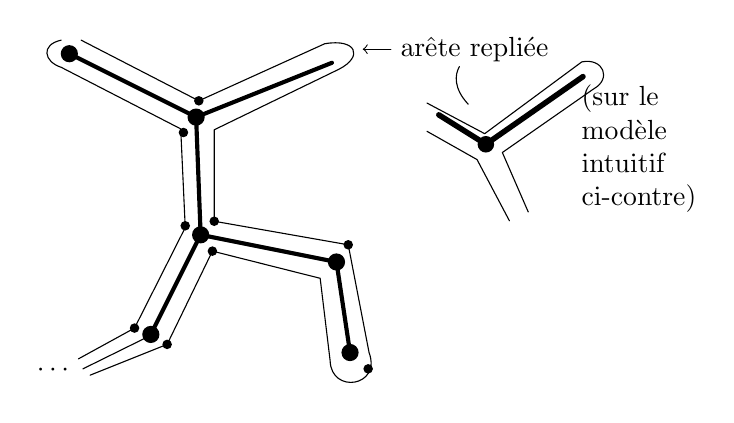
\begin{tikzpicture}[scale=1.15,line cap=round,line join=round]
\draw[line width=1.5pt] (-1.4,2.6)--(0,1.9)--(1.5,2.5) (0,1.9)--(.05,.6)--(-.5,-.5) (.05,.6)--(1.55,.3)--(1.7,-.7);
\draw (-1.49,2.75) .. controls (-1.72,2.7) and (-1.68,2.51) .. (-1.49,2.45)--(-.17,1.77)--(-.12,.68)--(-.68,-.43)--(-1.3,-.77);
\draw (-1.27,2.75)--(.03,2.08)--(1.42,2.71) .. controls (1.77,2.77) and (1.85,2.57) .. (1.58,2.43)--(.2,1.76)--(.2,.75)--(1.68,.49)--(1.91,-.7) .. controls (2.05,-1.08) and (1.49,-1.16) .. (1.48,-.79)--(1.37,.12)--(.18,.42)--(-.32,-.61)--(-1.17,-.95);
\draw (-1.25,-.88)--(-.52,-.52);
\foreach \x/\y in {-1.4/2.6,0/1.9,.05/.6,-.5/-.5,1.55/.3,1.7/-.7}{\fill (\x,\y) circle (2.7pt);}
\foreach \x/\y in {-.14/1.73,.03/2.08,-.12/.7,.2/.75,.18/.42,-.68/-.43,-.32/-.61,1.68/.49,1.9/-.88}{\fill (\x,\y) circle (1.5pt);}
\node at (-1.58,-.9) {$\cdots$};
\draw[<-] (1.84,2.65)--(2.15,2.65);\node[anchor=west] at (2.15,2.65) {arête repliée};
\begin{scope}[shift={(3.2,1.6)},scale=.65]
\draw[line width=2pt] (-.8,.5)--(0,0)--(1.65,1.15);
\fill (0,0) circle (4pt);
\draw (-1,.7)--(-.02,.18)--(1.63,1.4) .. controls (2,1.47) and (2.14,1.11) .. (1.83,.94)--(.28,-.14)--(.72,-1.15);
\draw (-1,.22)--(-.15,-.26)--(.4,-1.3);
\draw (-.3,.68) .. controls (-.55,.95) and (-.53,1.18) .. (-.45,1.32);
\end{scope}
\node[align=left,anchor=west] at (4.15,1.55) {(sur le\\modèle\\intuitif\\ci-contre)};
\end{tikzpicture}}
\margin{les sommets marqués sont marqués en gros, le contour de la découpe $D(X/K)$ en trait fin, les sommets sur le bord de la découpe sont \deleted{\unsure{tous}} figurés aussi.}

On reformule directement les axiomes en termes de $S\subset K\subset X$. Du point de vue des repères le long d'une arête pliée il y a deux repères (au lieu de quatre comme dans le cas précédemment étudié)

\mspage{55}
